\documentclass[12pt,a4paper]{article}

% --- Paquetes Recomendados ---
\usepackage[utf8]{inputenc}
\usepackage[spanish,es-tabla]{babel}
\usepackage{amsmath}
\usepackage{amsfonts}
\usepackage{amssymb}
\usepackage{graphicx}
\usepackage{geometry}
\usepackage{booktabs}
\usepackage{hyperref}
\usepackage{cite}
\usepackage{microtype}

% --- Configuración de Página ---
\geometry{left=3cm, right=3cm, top=2.5cm, bottom=2.5cm}

% --- Configuración de Enlaces ---
\hypersetup{
    colorlinks=true,
    linkcolor=blue,
    filecolor=magenta,      
    urlcolor=cyan,
    pdftitle={DIPAS: Diseño Inverso de Perfiles Aerodinámicos},
    pdfpagemode=FullScreen,
}

% --- Metadatos del Documento ---
\title{\textbf{DIPAS: Sistema de Diseño Generativo Inverso de Perfiles Aerodinámicos mediante CVAE y Validación Experimental}}
\author{\textbf{Julián} \\ \small Facultad de Ingeniería}
\date{\today}

\begin{document}

\maketitle

\begin{abstract}
Este trabajo presenta el desarrollo de DIPAS (DIseño de Perfiles AeroDinámicos Inverso), una metodología generativa basada en un Autoencoder Variacional Condicional (CVAE) para el diseño inverso de perfiles alares 2D en régimen subsónico incompresible. A diferencia de las metodologías tradicionales de optimización iterativa, el sistema propuesto mapea de forma directa las características de performance deseadas (coeficientes aerodinámicos y espesor relativo) a una geometría válida parametrizada mediante CST. El entrenamiento se realiza bajo un esquema multificidad combinando miles de simulaciones rápidas de XFOIL con datos RANS de alta fidelidad de AirfRANS. Finalmente, se propone una validación experimental en túnel de viento para cuantificar el salto entre la simulación numérica y la física real.
\end{abstract}

\newpage
\tableofcontents
\newpage

% --- Secciones del Documento ---
\section{Introducción}
\label{sec:introduccion}

El diseño aerodinámico de perfiles alares ha seguido tradicionalmente un enfoque directo, donde un diseñador propone una geometría inicial (por ejemplo, perfiles parametrizados de la serie NACA) y posteriormente evalúa su comportamiento mediante herramientas de mecánica de fluidos computacional (CFD) o ensayos experimentales. Este ciclo directo es inherentemente iterativo, lo que genera cuellos de botella significativos cuando se buscan óptimos locales bajo múltiples restricciones físicas.

\subsection{Objetivo del Proyecto}
El proyecto \textbf{DIPAS} (Diseño Inverso de Perfiles Aerodinámicos) tiene como objetivo subvertir este paradigma mediante el uso de aprendizaje profundo generativo. El usuario define un conjunto de objetivos de performance aerodinámica (tales como sustentación, resistencia y restricciones de espesor relativo a un número de Reynolds dado) y el modelo generativo genera de forma directa las coordenadas geométricas del perfil alar óptimo.

\subsection{Alcance y Límites del Trabajo}
Para garantizar la viabilidad técnica y experimental del proyecto, se delimitan los siguientes límites operativos:
\begin{itemize}
    \item \textbf{Dimensión}: Análisis estrictamente bidimensional (2D), ignorando efectos de envergadura finita o interacciones con fuselajes.
    \item \textbf{Régimen}: Subsónico e incompresible. El modelo se diseña para números de Reynolds moderados y bajos, típicos de vehículos aéreos no tripulados (UAVs) y aviación general ligera.
    \item \textbf{Flujo}: Estacionario, despreciando efectos dinámicos como desprendimiento dinámico o inestabilidades de capa límite transitorias.
\end{itemize}
Estos límites se definen formalmente como el marco conceptual del presente trabajo y no como omisiones de diseño.

\section{Metodología y Fundamentos Teóricos}
\label{sec:metodologia}

En esta sección se describen los pilares teóricos y conceptuales que sustentan el sistema DIPAS, detallando el funcionamiento de las redes neuronales generativas seleccionadas, el método de parametrización geométrica y la integración de todas las herramientas dentro del pipeline de diseño inverso.

\subsection{Modelos Generativos de Aprendizaje Profundo}
El diseño inverso en aerodinámica requiere mapear un espacio de requerimientos de performance unidimensionales a un espacio bidimensional geométrico complejo. Para lograr esto, se recurre a arquitecturas generativas capaces de aprender distribuciones probabilísticas de formas.

\subsubsection{Autoencoders (AE): La Idea Madre}
Un autoencoder es una arquitectura de red neuronal feed-forward diseñada para aprender representaciones eficientes de datos de entrada sin supervisión. El flujo de información se divide en dos bloques en cadena:
\begin{enumerate}
    \item \textbf{Codificador (Encoder)}: Comprime los datos de entrada de alta dimensión (en este caso, las coordenadas físicas del perfil alar descritas por cientos de puntos $x,y$) a una representación abstracta de muy baja dimensión, denominada \textit{espacio latente} ($z$).
    \item \textbf{Decodificador (Decoder)}: Toma el vector comprimido del espacio latente y busca reconstruir los datos originales con la menor pérdida de información posible.
\end{enumerate}
Este proceso es conceptualmente análogo a una parametrización geométrica clásica. Sin embargo, en lugar de que un diseñador humano defina el significado físico de cada parámetro, la red neuronal aprende de forma autónoma a identificar las características más significativas que resumen y diferencian la forma de los perfiles durante el entrenamiento.

\subsubsection{Autoencoders Variacionales (VAE): Generación de Nuevas Formas}
A diferencia de un autoencoder tradicional, el cual tiende a sobreajustarse y solo reconstruye de manera discreta los datos observados en el entrenamiento, el Autoencoder Variacional (VAE) introduce una restricción probabilística en el espacio latente. En lugar de mapear una entrada a un punto fijo en el espacio latente, el codificador de un VAE mapea la entrada a los parámetros de una distribución de probabilidad (usualmente una distribución Gaussiana con media $\mu$ y desviación estándar $\sigma$).

La función de pérdida incluye el término de divergencia de Kullback-Leibler ($\mathcal{D}_{KL}$), que penaliza la desviación del espacio latente respecto a una distribución prior estándar:
\begin{equation}
    \mathcal{L}_{VAE} = \mathcal{L}_{reconstruccion} + \beta \mathcal{D}_{KL}(q(z|x) \parallel p(z))
\end{equation}
Esta restricción matemática fuerza al espacio latente a organizarse de manera continua y suave (regularización). Como resultado, perfiles con geometrías similares se ubican en regiones contiguas del "mapa" latente. Para generar un perfil completamente nuevo, basta con muestrear un punto aleatorio dentro de este espacio latente continuo y procesarlo a través del decodificador.

\subsubsection{Autoencoders Variacionales Condicionales (CVAE): Diseño Objetivo}
Un VAE tradicional genera perfiles coherentes pero aleatorios, sin control directo sobre sus propiedades aerodinámicas. El Autoencoder Variacional Condicional (CVAE) \cite{wang2025cvae} resuelve esta limitación introduciendo un vector de condiciones $c$ concatenado tanto a la entrada del codificador como del decodificador.

En el sistema DIPAS, el vector de condiciones se define como un tensor cuatridimensional:
\begin{equation}
    c = \left[ Re_{norm}, C_{L,norm}, C_{D,norm}, (t/c)_{norm} \right]^T \in \mathbb{R}^4
\end{equation}
donde cada variable es normalizada linealmente al rango $[0, 1]$ a partir de los extremos del espacio de diseño ($Re \in [50{,}000, 300{,}000]$, $C_L \in [-0.2, 1.5]$, $C_D \in [0.005, 0.080]$, $t/c \in [0.06, 0.22]$).

\paragraph{Arquitectura y Dimensionalidad Latente}
A través de un estudio exhaustivo de ablación de hiperparámetros, se determinó que una dimensionalidad del espacio latente de $z \in \mathbb{R}^6$ ofrece el equilibrio óptimo entre compresión de datos y capacidad de representación, evitando tanto el subajuste como el colapso de información. 
La red está compuesta por:
\begin{itemize}
    \item \textbf{Codificador}: Capas densas secuenciales de $[256, 128, 64]$ neuronas con activación LeakyReLU ($\alpha = 0.2$) y Batch Normalization, que proyectan el vector concatenado de $12\text{ CST} + 4\text{ condiciones} = 16$ variables a los vectores de parámetros Gaussianos $\mu \in \mathbb{R}^6$ y $\log(\sigma^2) \in \mathbb{R}^6$.
    \item \textbf{Decodificador}: Capas densas simétricas de $[64, 128, 256]$ neuronas que toman el vector latente muestreado $z$ junto con las condiciones $c$ ($6 + 4 = 10$ entradas) y reconstruyen los $12$ coeficientes CST del perfil alar ($a = [a^u, a^l]$).
\end{itemize}

\paragraph{Función de Pérdida Compuesta con Regularización Geométrica}
Para asegurar que los coeficientes generados produzcan formas aerodinámicamente suaves y sin intersecciones, se formuló una función de pérdida híbrida diferenciable:
\begin{equation}
    \mathcal{L}_{CVAE} = \mathcal{L}_{CST} + w_{geom} \cdot \mathcal{L}_{coords} + \beta \cdot \mathcal{D}_{KL}
\end{equation}
donde $\mathcal{L}_{CST} = \frac{1}{12} \sum_{i=1}^{12} (a_i - \hat{a}_i)^2$ es el error cuadrático medio en los coeficientes, $\mathcal{L}_{coords} = \frac{1}{200} \sum_{j=1}^{200} (y_j - \hat{y}_j)^2$ es el error geométrico directo en las coordenadas físicas del perfil calculado en tiempo real por la capa diferenciable CST, $w_{geom} = 20.0$ es el factor de ponderación geométrica, y $\beta = 0.01$ modula la regularización de Kullback-Leibler.

\subsection{Arquitecturas Alternativas: Redes Neuronales Generativas Adversarias (GAN)}
Un enfoque alternativo al CVAE son las Redes Generativas Adversarias (GAN). Esta arquitectura carece de un codificador explícito y basa su entrenamiento en la competencia de dos redes neuronales distintas:
\begin{itemize}
    \item \textbf{El Generador}: Intenta crear geometrías sintéticas de perfiles alares a partir de ruido aleatorio para engañar al discriminador.
    \item \textbf{El Discriminador}: Clasifica si una geometría de perfil alar proviene del dataset real de entrenamiento o si fue inventada por el generador.
\end{itemize}

Ambas redes se entrenan de forma simultánea en un juego de suma cero. Aunque las GANs (como las variantes conditional GAN o WGAN-gp) son altamente eficaces produciendo perfiles con un alto grado de suavidad y diversidad geométrica, presentan dificultades de entrenamiento (como el colapso de modo) y requieren un volumen de datos sustancialmente mayor para converger. 

\subsubsection{Justificación del Uso de CVAE frente a GAN}
Para DIPAS, se seleccionó la arquitectura CVAE por las siguientes razones de ingeniería:
\begin{itemize}
    \item \textbf{Eficiencia de Datos}: El CVAE presenta una convergencia más estable y requiere menos datos de entrenamiento que una GAN, siendo la opción más robusta para el alcance de un proyecto de grado con limitaciones computacionales.
    \item \textbf{Precisión del Condicionamiento}: La literatura científica reporta que los CVAE son más precisos para reproducir los valores específicos de la condición de entrada (por ejemplo, el coeficiente de sustentación objetivo $C_L$) en comparación con las GAN, las cuales priorizan la suavidad visual sobre la exactitud de las restricciones físicas de entrada.
\end{itemize}

\subsection{Parametrización Geométrica mediante CST}
La parametrización de perfiles mediante la técnica de Transformación de Clase y Forma (CST, por sus siglas en inglés \textit{Class Shape Transformation}) no es un modelo de aprendizaje automático, sino un método analítico de representación de curvas de frontera.

CST describe la geometría de la superficie superior ($y_u$) e inferior ($y_l$) de un perfil mediante la multiplicación de una función de clase $C(x)$ (que establece la topología general del perfil, como bordes de ataque redondeados y bordes de fuga afilados) y una función de forma $S(x)$ (compuesta por polinomios de Bernstein escalados por pesos de control $a_i$):
\begin{equation}
    y_u(x) = C(x) \cdot S_u(x) + x \cdot \frac{\Delta t_{te}}{2}
\end{equation}
\begin{equation}
    y_l(x) = C(x) \cdot S_l(x) - x \cdot \frac{\Delta t_{te}}{2}
\end{equation}
donde $\Delta t_{te}$ es el espesor de diseño en el borde de fuga.

### Función de Clase
La función de clase actúa como un envolvente geométrico que restringe los extremos del perfil a cerrarse en valores físicos precisos. Se define matemáticamente como:
\begin{equation}
    C(x) = x^{0.5} \cdot (1 - x)^{1.0}
\end{equation}
Dado que $C(0) = 0$ y $C(1) = 0$, esta función obliga a que las coordenadas finales del perfil comiencen en el origen y se cierren en el extremo del borde de fuga, sin importar el valor de la función de forma. La raíz cuadrada ($x^{0.5}$) introduce una pendiente vertical en el origen, garantizando un borde de ataque redondeado y suave.

### Función de Forma y Polinomios de Bernstein
La función de forma $S(x)$ se representa como una combinación lineal de polinomios de Bernstein de orden $n$:
\begin{equation}
    S(x) = \sum_{i=0}^{n} a_i \cdot B_{i,n}(x)
\end{equation}
donde $a_i$ representan los coeficientes (pesos) de diseño. Los polinomios de Bernstein base de grado $n$ se definen como:
\begin{equation}
    B_{i,n}(x) = \binom{n}{i} x^i (1 - x)^{n - i}
\end{equation}
Para un orden $n = 5$ (lo que genera $6$ coeficientes por superficie), los polinomios base se muestran en la Fig.~\ref{fig:bernstein_basis}. Estos polinomios cuentan con la propiedad de partición de la unidad ($\sum_{i=0}^{n} B_{i,n}(x) = 1$), lo que los hace ideales para representar variaciones relativas de espesor de manera normalizada.

\begin{figure}[htbp]
    \centering
    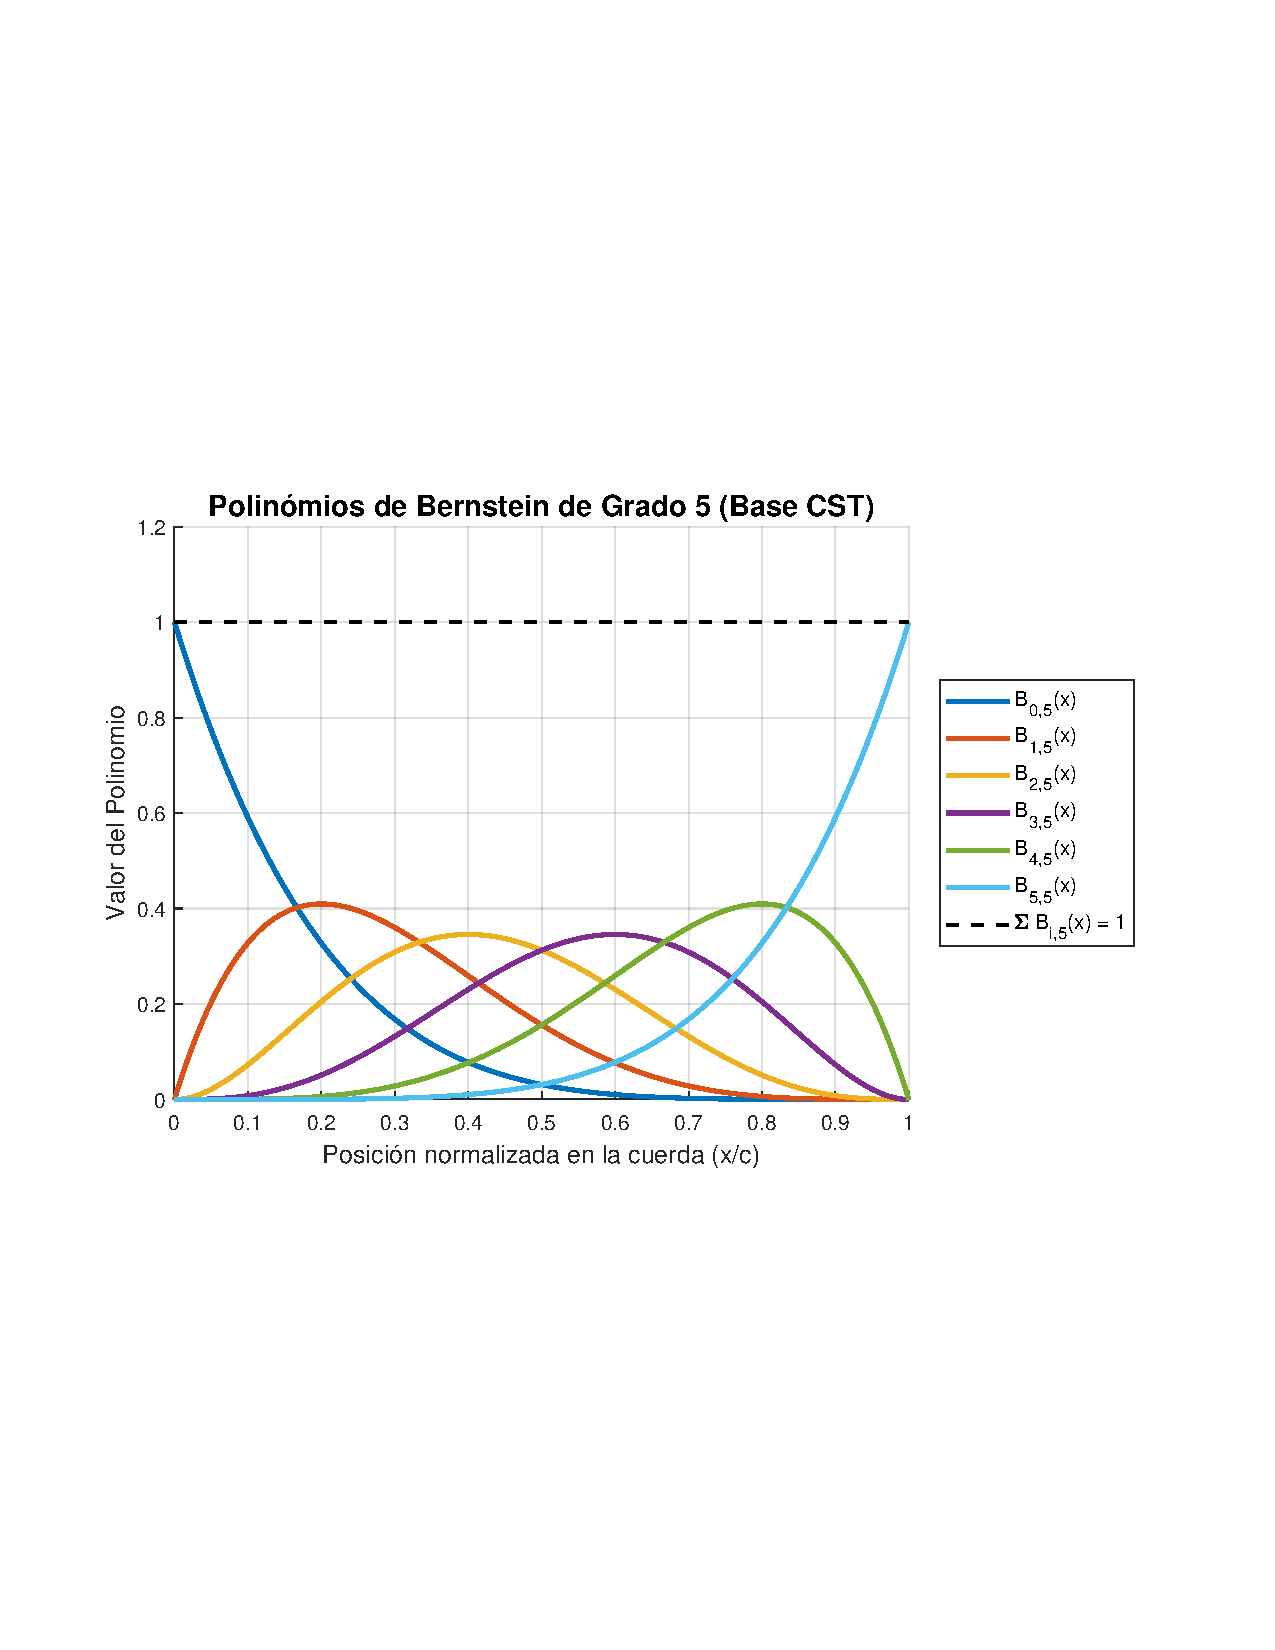
\includegraphics[width=0.85\textwidth]{figures/bernstein_basis.pdf}
    \caption{Polinomios de Bernstein de grado 5 utilizados como base en el método CST.}
    \label{fig:bernstein_basis}
\end{figure}

El uso de polinomios de Bernstein aporta una ventaja de diseño crítica: el \textbf{control local}. Como cada polinomio de la base tiene su pico de influencia en una posición de cuerda específica (por ejemplo, $B_{0,5}$ en el borde de ataque, $B_{5,5}$ en el borde de fuga, y los intermedios distribuidos linealmente), modificar un coeficiente $a_i$ específico solo deforma de manera suave la región local correspondiente sin alterar el resto del perfil, como se ilustra en la Fig.~\ref{fig:cst_components}.

\begin{figure}[htbp]
    \centering
    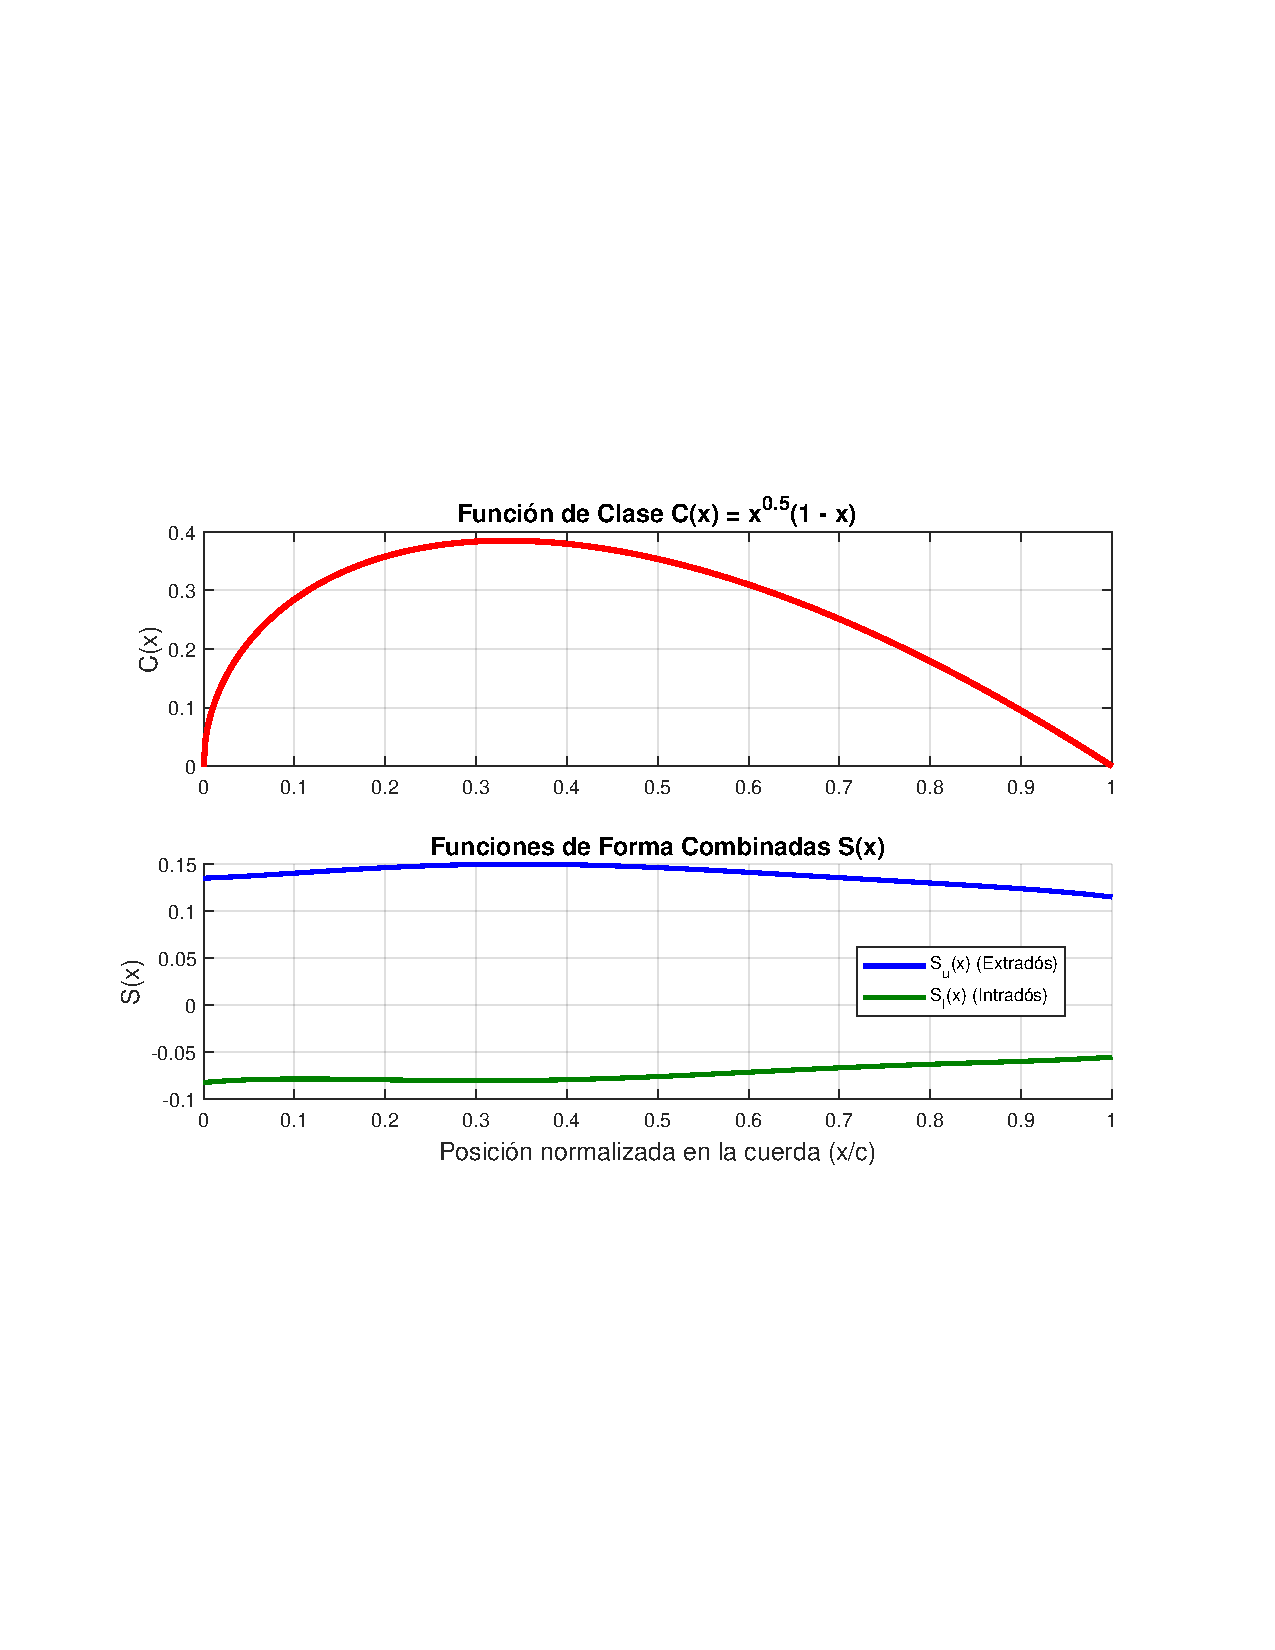
\includegraphics[width=0.85\textwidth]{figures/cst_components.pdf}
    \caption{Función de clase $C(x)$ (arriba) y funciones de forma resultantes $S_u(x)$ y $S_l(x)$ (abajo) para la reconstrucción de un perfil Selig S3021.}
    \label{fig:cst_components}
\end{figure}

Al multiplicar ambas funciones, se obtiene el perfil alar completo mostrado en la Fig.~\ref{fig:reconstructed_airfoil}.

\begin{figure}[htbp]
    \centering
    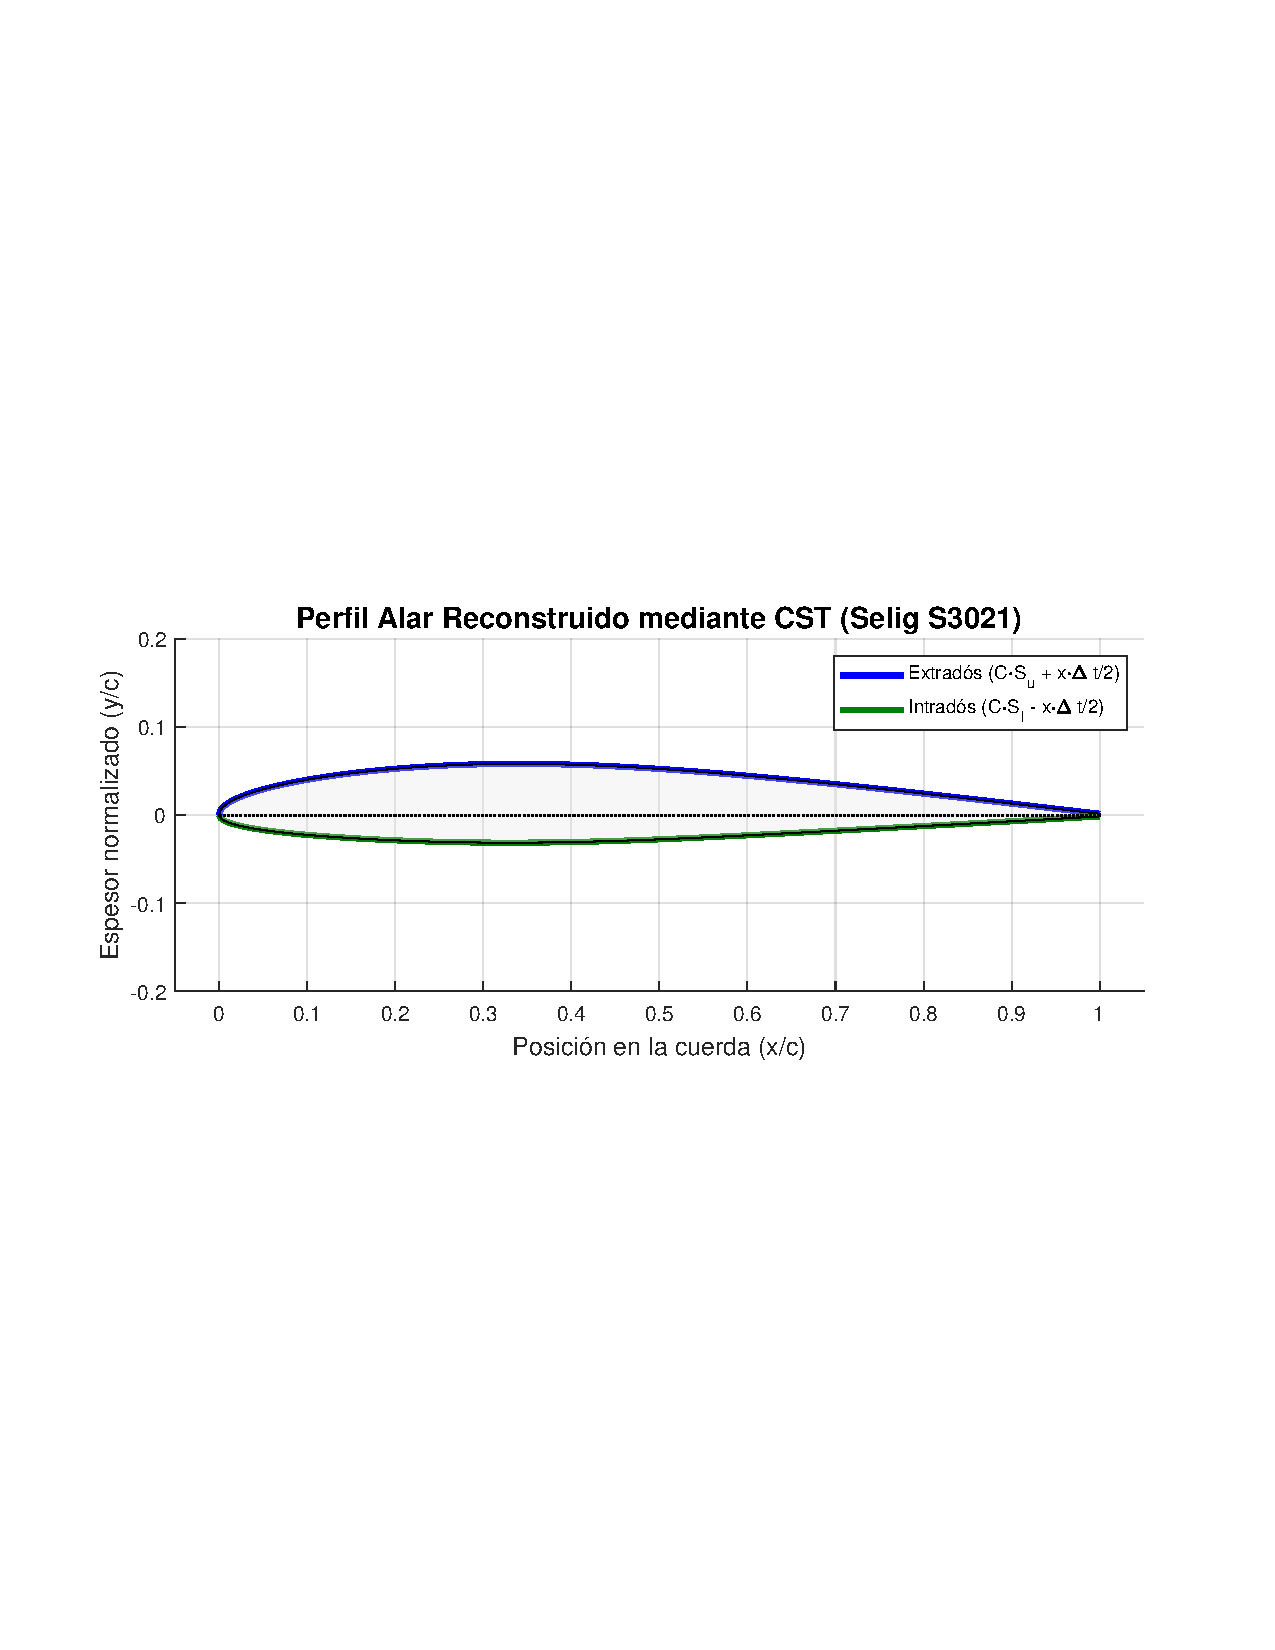
\includegraphics[width=0.95\textwidth]{figures/reconstructed_airfoil.pdf}
    \caption{Perfil alar final Selig S3021 reconstruido a partir de la multiplicación $C(x) \cdot S(x)$.}
    \label{fig:reconstructed_airfoil}
\end{figure}

El vector de pesos final $a = [a^u, a^l]$ resume la compleja geometría de entrada de cientos de coordenadas en una firma digital compacta de 12 variables continuas, facilitando la convergencia del modelo generativo.

### Ajuste de Coeficientes mediante Mínimos Cuadrados Lineales
Dado que se busca transformar perfiles reales existentes de la base de datos a su representación en coeficientes CST, se define un problema de optimización lineal. Para un conjunto de $M$ puntos de coordenadas conocidas $(x_j, y_{real,j})$ (típicamente $M \approx 100$), el sistema de ecuaciones para el extradós es de la forma:
\begin{equation}
    y_{real}(x_j) \approx C(x_j) \cdot \sum_{i=0}^{n} a_i B_{i,n}(x_j)
\end{equation}
Al contar con $M$ ecuaciones y solo $n+1$ incógnitas ($6$ coeficientes por superficie), el sistema lineal está sobredeterminado y se escribe matricialmente como:
\begin{equation}
    Y = A \cdot a + e
\end{equation}
donde $Y \in \mathbb{R}^{M \times 1}$ es el vector de coordenadas reales, $A \in \mathbb{R}^{M \times (n+1)}$ es la matriz de diseño evaluada en cada punto $x_j$, $a \in \mathbb{R}^{(n+1) \times 1}$ es el vector de coeficientes incógnita y $e \in \mathbb{R}^{M \times 1}$ es el vector de errores o residuos locales. Los elementos de la matriz $A$ están definidos por:
\begin{equation}
    A_{j,i} = C(x_j) \cdot B_{i,n}(x_j)
\end{equation}

El algoritmo busca encontrar el vector de coeficientes $a$ que minimice la suma de los errores al cuadrado (norma residual L2):
\begin{equation}
    E(a) = \sum_{j=1}^{M} e_j^2 = \|Y - A \cdot a\|^2
\end{equation}
Para minimizar $E(a)$, se deriva la función de error respecto a cada coeficiente $a_i$ e iguala a cero, obteniendo las llamadas \textit{Ecuaciones Normales}:
\begin{equation}
    A^T A \cdot a = A^T Y
\end{equation}
Dado que la matriz reducida $A^T A \in \mathbb{R}^{(n+1) \times (n+1)}$ es cuadrada y de rango completo, se puede resolver directamente multiplicando por su inversa (pseudo-inversa de Moore-Penrose):
\begin{equation}
    a = (A^T A)^{-1} A^T Y
\end{equation}
Este método analítico asegura que el perfil CST generado tenga la mínima desviación cuadrática media respecto al perfil real, garantizando un error típico de ajuste inferior a $10^{-6}$ en escala adimensional. La validación práctica de este ajuste se presenta en la Fig.~\ref{fig:reconstructed_cst_fit}, donde se contrasta la geometría del perfil real Selig S3021 frente a la reconstrucción paramétrica obtenida usando 12 coeficientes CST.

\begin{figure}[htbp]
    \centering
    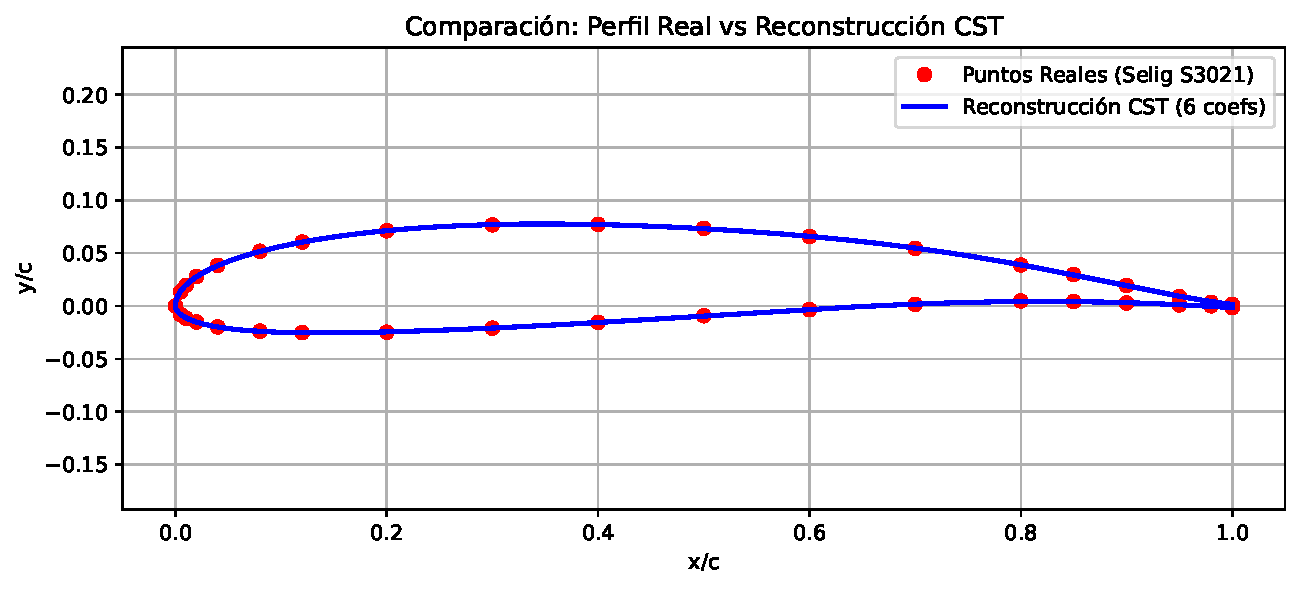
\includegraphics[width=0.95\textwidth]{figures/reconstructed_cst_fit.pdf}
    \caption{Validación del ajuste por mínimos cuadrados de un perfil Selig S3021 utilizando 12 coeficientes CST.}
    \label{fig:reconstructed_cst_fit}
\end{figure}

\subsubsection{Capa Diferenciable CST en PyTorch (CSTCoordinateLayer)}
\label{subsubsec:cst_layer}
Para permitir que las redes generativas y sustitutas calculen pérdidas geométricas y espesores en tiempo real dentro del grafo computacional de PyTorch (sin recurrir a llamadas externas de CPU en NumPy), se implementó un módulo personalizado totalmente diferenciable denominado \texttt{CSTCoordinateLayer}.

\paragraph{Formulación Matricial y Buffers Constantes}
La capa precalcula una grilla de coseno de $N=100$ puntos $\theta_j \in [0, \pi] \implies x_j = \frac{1}{2}(1 - \cos\theta_j)$, la función de clase $C(x) \in \mathbb{R}^{1 \times N}$, y las matrices de polinomios de Bernstein base para el extradós e intradós:
\begin{equation}
    B_u \in \mathbb{R}^{n_u \times N}, \quad B_l \in \mathbb{R}^{n_l \times N}
\end{equation}
donde cada elemento $B_{i, j} = \binom{n-1}{i} x_j^i (1 - x_j)^{n - 1 - i}$ se almacena en memoria como un buffer constante no entrenable (\texttt{register\_buffer}) alojado directamente en el dispositivo de cómputo (GPU o CPU).

Durante el pase hacia adelante (\textit{forward pass}), para un lote de coeficientes predichos $a^u \in \mathbb{R}^{B \times n_u}$ y $a^l \in \mathbb{R}^{B \times n_l}$, las funciones de forma continuas se obtienen mediante multiplicaciones de matrices vectorizadas de alta velocidad:
\begin{equation}
    S_u = a^u \cdot B_u \in \mathbb{R}^{B \times N}, \quad S_l = a^l \cdot B_l \in \mathbb{R}^{B \times N}
\end{equation}
Las coordenadas físicas superiores e inferiores se sintetizan de forma exacta y diferenciable:
\begin{equation}
    y_u = C(x) \odot S_u + x \cdot \frac{\Delta t_{te}}{2}, \quad y_l = C(x) \odot S_l - x \cdot \frac{\Delta t_{te}}{2}
\end{equation}
donde $\odot$ denota el producto elemento a elemento de Hadamard. La diferenciabilidad analítica de esta capa permite propagar el gradiente exacto $\frac{\partial \mathcal{L}_{coords}}{\partial a}$ directamente hacia los pesos del decodificador y hacia el vector latente $z$.



\subsection{Integración de Componentes en DIPAS}
El flujo de diseño y entrenamiento de DIPAS conecta de forma secuencial las herramientas descritas:
\begin{enumerate}
    \item \textbf{CST} se utiliza como la herramienta generadora de variantes: se toman perfiles reales de la base de datos UIUC, se ajustan sus coeficientes CST y se aplican perturbaciones controladas para generar miles de geometrías nuevas pero físicamente coherentes.
    \item \textbf{XFOIL} evalúa rápidamente estas miles de geometrías en un barrido de ángulos de ataque y números de Reynolds, aportando las polares de coeficientes ($C_L, C_D, C_M$) que compondrán las etiquetas de entrenamiento.
    \item El \textbf{CVAE} se entrena con esta base de datos masiva para aprender la función inversa: generar el vector de coeficientes CST (geometría) a partir de los coeficientes de performance condicionados ($C_L, C_D, Re, t/c$).
\subsection{Justificación Física del Enfoque Multifidelidad: Limitaciones de XFOIL vs. ANSYS Fluent}
\label{subsec:justificacion_multifidelidad}

El diseño aerodinámico asistido por Inteligencia Artificial en regímenes de bajo número de Reynolds ($Re = 50{,}000 - 200{,}000$) presenta desafíos físicos particulares derivados de la fuerte sensibilidad de la capa límite laminar y la formación de burbujas de separación laminar (\textit{Laminar Separation Bubbles}, LSB). En este régimen, los métodos clásicos de paneles con capa límite integral (como XFOIL) presentan limitaciones fundamentales que justifican la adopción de una metodología multifidelidad combinada con simulaciones Navier-Stokes (RANS) de alta fidelidad en ANSYS Fluent.

\subsubsection{Comparativa Física de Modelos de Simulación}
En el Cuadro~\ref{tab:xfoil_vs_ansys} se resumen las principales diferencias teóricas y numéricas entre el resolvedor de baja fidelidad (XFOIL) y el de alta fidelidad (ANSYS Fluent con modelo \textit{Transition SST} $\gamma\text{-}Re_\theta$).

\begin{table}[htbp]
\centering
\small
\caption{Comparación física y numérica entre XFOIL y ANSYS Fluent en régimen de bajo Reynolds.}
\label{tab:xfoil_vs_ansys}
\begin{tabular}{p{3.2cm} p{4.2cm} p{4.2cm} p{3.2cm}}
\toprule
\textbf{Fenómeno} & \textbf{XFOIL (Método Integral 1D)} & \textbf{ANSYS Fluent (Transition SST $\gamma\text{-}Re_\theta$)} & \textbf{Impacto Físico en el Diseño} \\
\midrule
\textbf{Ecuaciones resueltas} & Integrales promediadas 1D en la superficie del perfil. & Navier-Stokes 2D promediadas (RANS) en todo el dominio fluido. & ANSYS captura la recirculación y vorticidad real dentro de la burbuja. \\
\addlinespace
\textbf{Burbujas cortas ($Re > 200{,}000$)} & Buena aproximación general. & Alta precisión cuantitativa. & Error menor en $C_L$, leve subestimación de $C_D$ en XFOIL. \\
\addlinespace
\textbf{Burbujas largas ($Re \le 100{,}000$)} & Falla o no converge. Asume capa límite delgada (violación de hipótesis). & Modela la deformación real del campo de presiones ($C_p$). & XFOIL predice desprendimientos irreales o diverge numéricamente. \\
\addlinespace
\textbf{Gradientes de presión y curvatura} & Aproximación parabólica simplificada. & Tensor de tensiones de Reynolds completo ($4$ ecuaciones). & ANSYS predice con exactitud la meseta (\textit{plateau}) de presión. \\
\addlinespace
\textbf{Predicción de Arrastre ($C_D$)} & Subestima $C_D$ típicamente entre $15\%$ y $35\%$. & Ajuste muy preciso con datos de túnel de viento UIUC. & La energía disipada por el vórtice de la burbuja no se capta en 1D. \\
\bottomrule
\end{tabular}
\end{table}

\subsubsection{Impacto en el Proceso de Diseño Aerodinámico}
Las discrepancias señaladas afectan de manera crítica tres aspectos fundamentales del perfil generado:
\begin{enumerate}
    \item \textbf{Subestimación del Arrastre Total ($C_D$)}: Optimizar un perfil puramente con XFOIL a $Re = 100{,}000$ puede arrojar un $C_D = 0.012$; no obstante, al ensayarlo experimentalmente o simularlo en RANS, el arrastre real asciende a $C_D = 0.016 - 0.018$ (un incremento del $30\%$ debido a la disipación viscosa y pérdidas de presión en la recirculación de la burbuja).
    \item \textbf{Histéresis y No Linealidades en la Polar}: La formación, crecimiento y reatachamiento de la burbuja laminar introduce ondulaciones no lineales en la curva $C_L$ vs $\alpha$. XFOIL suele suavizar artificialmente estas transiciones o fallar por no convergencia en los ángulos críticos de transición.
    \item \textbf{Desprendimiento Prematuro y Alteración de Momento ($C_M$)}: A ángulos de ataque moderados ($\alpha \ge 6^\circ - 8^\circ$), el desplazamiento de la burbuja hacia el borde de ataque altera drásticamente la distribución de presiones $C_p$, modificando el momento de cabeceo y la estabilidad estática del UAV.
\end{enumerate}

\subsubsection{Justificación de la Estrategia Multifidelidad en DIPAS}
La conjunción de estos factores fundamenta el diseño de la arquitectura generativa propuesta:
\begin{itemize}
    \item \textbf{Baja Fidelidad (XFOIL / UniFoil)}: Permite explorar de forma masiva y a costo computacional casi nulo (milisegundos) el espacio morfológico global ($146{,}000$ muestras).
    \item \textbf{Alta Fidelidad (ANSYS Fluent Transition-SST)}: Corrige la física local de la burbuja de separación laminar y calibra con precisión milimétrica el coeficiente de arrastre real.
    \item \textbf{CVAE + Surrogate Híbrido}: Aprende a fusionar ambos niveles de fidelidad, ofreciendo la velocidad de inferencia de una red neuronal profunda con la rigurosidad física de un solver Navier-Stokes de última generación.
\end{itemize}

\subsection{Automatización CFD de Alta Fidelidad y Dataset de Ajuste Fino}
\label{subsec:automatizacion_cfd}

Para el ajuste fino (\textit{fine-tuning}) del modelo generativo CVAE con física de alta fidelidad, se desarrolló e implementó un pipeline de automatización numérica en lote (\textit{batch}) que acopla de manera desatendida las herramientas de simulación de ANSYS Suite 2026 R1 (SpaceClaim, Meshing y Fluent) mediante scripts en Python. Este proceso permitió generar un dataset secundario de alta fidelidad compuesto por $1{,}000$ simulaciones CFD completas ($125$ variantes de perfiles $\times$ $8$ ángulos de ataque).

\subsubsection{Reconstrucción CAD y Remallado Dinámico en Batch}
La actualización geométrica tradicional en ANSYS Workbench suele ser propensa a fallos de asociación cuando las Named Selections pierden referencia al cambiar la nube de puntos del perfil. Para superar esta limitación, el script de control principal \texttt{wb\_run\_spaceclaim\_update.py} ejecuta el siguiente flujo automatizado en segundo plano utilizando el motor de comandos de Workbench y SpaceClaim:
\begin{enumerate}
    \item \textbf{Carga del Proyecto Schematic}: Se abre el proyecto base con la API de Workbench.
    \item \textbf{Scripting en SpaceClaim}: Se envían comandos de geometría en Python de SpaceClaim para:
        \begin{itemize}
            \item Borrar los cuerpos y curvas del perfil de la corrida previa.
            \item Importar la nueva nube de coordenadas del perfil perturbado mediante CST y generar la cara sólida del perfil en 2D.
            \item Dibujar un dominio fluido rectangular exterior de $7.0\text{ m} \times 6.0\text{ m}$.
            \item Realizar la operación booleana de sustracción (dominio exterior menos perfil alar) para obtener el dominio fluido final.
            \item Identificar y asignar dinámicamente las entidades geométricas a sus respectivos grupos de Named Selections (\texttt{inlet}, \texttt{outlet}, \texttt{symmetry}, \texttt{airfoil} y \texttt{fluid}) basándose en la posición espacial de los bordes.
        \end{itemize}
    \item \textbf{Exportación de Malla Mediante API Directa de Meshing}: En lugar de utilizar la celda de actualización estándar de Workbench (que suele omitir la escritura física en disco), se inicializa ANSYS Meshing de forma no interactiva y se inyecta un comando directo a la interfaz del modelo utilizando la API de scripting de Mechanical:
        \begin{equation}
            \texttt{mesh.InternalObject.WriteFluentInputFile(mesh\_path)}
        \end{equation}
        Esto fuerza al motor a regenerar la malla no estructurada y exportar físicamente un archivo limpio \texttt{FFF-1.msh} al directorio de trabajo en menos de 50 segundos.
\end{enumerate}

\subsubsection{Bucle de Simulación Polar en ANSYS Fluent}
Una vez generada la malla física, el orquestador en Python genera dinámicamente un archivo de comandos Journal (\texttt{run\_polar.jou}) para ejecutar un barrido polar de 8 ángulos de ataque ($\alpha = [-2, 0, 2, 4, 6, 8, 10, 12]^\circ$) en una única ejecución desatendida de ANSYS Fluent en paralelo.
\begin{itemize}
    \item \textbf{Modelo Físico}: Se selecciona el modelo de turbulencia de cuatro ecuaciones \textit{Transition SST} (\textit{Menter's Shear Stress Transport} con modelo de transición de capa límite) para capturar adecuadamente la burbuja de separación laminar a bajo número de Reynolds ($Re = 150{,}000$).
    \item \textbf{Bucle de Ángulos de Ataque}: Para cada ángulo $\alpha$, se recalculan las componentes vectoriales del flujo de entrada ($x$-component $= \cos\alpha$ e $y$-component $= \sin\alpha$) y se inyecta una secuencia exacta de 17 respuestas a los prompts del TUI de Fluent para cambiar las condiciones en el \texttt{velocity-inlet}.
    \item \textbf{Gestión de Inicialización y Memoria}: Para evitar bloqueos durante el barrido, se inyecta la confirmación \texttt{"ok"} para descartar la solución previa antes de ejecutar la inicialización híbrida (\texttt{hyb-initialization}). Asimismo, se eliminan los archivos de reporte del ángulo anterior de la memoria del solver utilizando el comando:
        \begin{equation}
            \texttt{/solve/report-files/delete cd-file-<idx-1>}
        \end{equation}
        evitando así prompts interactivos de sobrescritura de archivos que detengan la ejecución en batch.
\end{itemize}

\subsubsection{Robustez del Pipeline y Reanudación Automática}
El script final \texttt{dataset\_cfd\_builder.py} cuenta con un mecanismo de reanudación automática (\textit{check-pointing}) que analiza el archivo CSV de salida y salta instantáneamente los perfiles ya simulados. Para mitigar las excepciones por violación de acceso de archivos comunes en sistemas Windows (\texttt{WinError 32}) al cerrar procesos concurrentes, se incorporó una pausa de seguridad de $1.5\text{ s}$ después del cierre de Fluent, complementada por un bucle de hasta 5 intentos de lectura de datos con retardos discretos de $0.5\text{ s}$.

El dataset resultante, guardado de forma segura en \texttt{dataset\_cfd.csv}, contiene registros consistentes con la física de fluidos de transición de capa límite, listo para el entrenamiento del CVAE en la siguiente fase de desarrollo.

\subsection{Datasets Públicos del Estado del Arte y Estrategia de Transfer Learning}
\label{subsec:datasets_publicos}

Con el fin de posicionar el sistema DIPAS dentro del panorama científico contemporáneo, se realiza un relevamiento de los datasets públicos de aerodinámica de perfiles alares más relevantes del estado del arte, evaluando su utilidad para tareas de pre-entrenamiento, adaptación de bajo Reynolds y validación externa.

\subsubsection{Catálogo de Datasets Públicos de Referencia}
\begin{enumerate}
    \item \textbf{UniFoil (University of Tennessee, NeurIPS 2025)}: Es el dataset de CFD de perfiles alares 2D más masivo disponible. Cuenta con más de $500{,}000$ simulaciones sobre aproximadamente $30{,}000$ perfiles únicos en regímenes variados de Mach y Reynolds, incluyendo coeficientes globales ($C_L$, $C_D$, $C_M$), distribución de presiones ($C_p$) y datos de transición.
    \item \textbf{UIUC Low-Reynolds Airfoil Data (University of Illinois Urbana-Champaign)}: Recopilación histórica y estándar de ensayos experimentales en túnel de viento para perfiles a bajos números de Reynolds ($Re = 100{,}000\text{ a }500{,}000$). Aporta curvas polares físicas reales ($C_L, C_D, C_M$).
    \item \textbf{Dataset CST (Kanakaero, 2024)}: Contiene $2{,}900$ perfiles parametrizados directamente con coeficientes CST y simulados a $Re = 100{,}000$, lo cual resulta conceptualmente idéntico a la representación geométrica de DIPAS.
    \item \textbf{CFD Database (Politecnico di Milano)}: Ofrece campos de flujo RANS 2D de alta resolución sobre $2{,}600$ geometrías NACA a altos números de Reynolds ($Re = 3 \times 10^6$).
    \item \textbf{100k Airfoil Pressure Dataset (Università Roma Tre)}: Reúne distribuciones de presión $C_p$ para $100{,}000$ geometrías mediante flujo potencial (método de paneles), representando una fuente de baja fidelidad conceptualmente análoga a XFOIL.
\end{enumerate}

La Tabla~\ref{tab:datasets_multifidelidad} detalla la estructura y el rol de cada una de estas bases de datos dentro de la arquitectura multificidad y multi-fuente de DIPAS.

\begin{table}[htbp]
\centering
\caption{Estructura, fidelidad y rol de los datasets integrados en DIPAS.}
\label{tab:datasets_multifidelidad}
\small
\begin{tabular}{@{}lllll@{}}
\toprule
\textbf{Fuente} & \textbf{Rango de Reynolds} & \textbf{Tipo de Datos} & \textbf{Fidelidad} & \textbf{Uso en DIPAS} \\ \midrule
UniFoil (NeurIPS) & $10^6\text{ a }10^7$ & CFD (RANS) & Media-Alta & Pre-entrenamiento General \\
UIUC (Illinois) & $10^5\text{ a }5\times 10^5$ & Experimental & Física Real & Adaptación LRN / Test Ciego \\
Dataset CST & $10^5$ & CFD + CST & Media & Adaptación Geométrica CST \\
DIPAS XFOIL & $10^5\text{ a }3\times 10^5$ & Panel + Capa Lím. & Baja-Media & Dataset Propio (Pre-train) \\
DIPAS Fluent & $10^5\text{ a }2\times 10^5$ & CFD (RANS Trans.) & Alta & Dataset Propio (Fine-tuning) \\
Túnel DIPAS & $1.5\times 10^5$ & Experimental & Física Real & Validación Experimental Final \\ \bottomrule
\end{tabular}
\end{table}

\subsubsection{La Escalera de Reynolds: Transfer Learning Progresivo}
Para diseñar de forma óptima a bajos números de Reynolds ($Re \approx 150{,}000$), donde la dinámica de fluidos está dominada por efectos viscosos de separación y transición laminar, no es conveniente entrenar un modelo generativo directamente con datos turbulentos de altos Reynolds, ni tampoco empezar desde cero con pocas simulaciones Fluent locales. 

En su lugar, DIPAS implementa una \textbf{Escalera de Reynolds} mediante aprendizaje por transferencia (\textit{Transfer Learning}) progresivo. El modelo aprende primero los principios universales de la sustentación y reconstrucción de formas en altos Reynolds, y luego desciende gradualmente hacia las sutilezas de la capa límite transicional a bajos Reynolds:

\begin{equation}
    Re \approx 10^7 \xrightarrow{\text{UniFoil}} Re \approx 10^5 \xrightarrow{\text{CST / UIUC}} Re \in [10^5, 3\cdot 10^5] \xrightarrow{\text{DIPAS XFOIL}} Re \in [10^5, 2\cdot 10^5] \xrightarrow{\text{DIPAS Fluent}}
\end{equation}

\begin{enumerate}
    \item \textbf{Paso 1: Pre-entrenamiento (UniFoil)}: Mapeo global de formas 2D y principios generales de sustentación/arrastre a altos números de Reynolds ($10^6\text{--}10^7$).
    \item \textbf{Paso 2: Adaptación de Bajo Reynolds (Kanakaero \& UIUC)}: Ajuste intermedio del espacio latente con geometrías ya mapeadas a coeficientes CST a $Re = 100{,}000$, introduciendo la respuesta experimental física real de la base de datos de la UIUC.
    \item \textbf{Paso 3: Ajuste Fino Propio de Baja Fidelidad (DIPAS XFOIL)}: Adaptación de la red a la respuesta transicional rápida sobre los $9{,}931$ perfiles ($146{,}916$ polares) parametrizados mediante CST a bajos Reynolds.
    \item \textbf{Paso 4: Calibración final de Alta Fidelidad (DIPAS Fluent)}: Ajuste fino definitivo sobre el dataset de RANS con modelo de transición de 4 ecuaciones ($Transition-SST$) a múltiples Reynolds ($100k, 150k, 200k$), garantizando que el modelo capture adecuadamente la burbuja de separación laminar.
\end{enumerate}

\subsubsection{Validación Externa y Pregunta de Investigación}
Para validar la capacidad de generalización del CVAE y del modelo sustituto (\textit{surrogate model}) de DIPAS, se separa un $20\%$ del dataset experimental de la UIUC de perfiles que el modelo jamás vio durante ninguna de las fases de entrenamiento. Se contrasta de forma directa:
\begin{equation}
    C_{L,\text{DIPAS}} \leftrightarrow C_{L,\text{UIUC (Exp)}} \quad \text{y} \quad C_{D,\text{DIPAS}} \leftrightarrow C_{D,\text{UIUC (Exp)}}
\end{equation}

Esto permite formular y responder de manera rigurosa la siguiente pregunta de investigación:
\begin{quote}
    \textit{¿El pre-entrenamiento aerodinámico multifidelidad y multi-fuente permite reducir la cantidad de simulaciones numéricas de alta fidelidad necesarias para construir un modelo generativo de diseño inverso preciso a bajos números de Reynolds?}
\end{quote}

Para responder a esto, se evaluará la tasa de error de reconstrucción y de predicción física del CVAE bajo cuatro escenarios experimentales de entrenamiento:
\begin{itemize}
    \item \textbf{Escenario A (DIPAS desde cero)}: Entrenamiento del CVAE usando únicamente el dataset local de XFOIL y Fluent de DIPAS.
    \item \textbf{Escenario B (CFD Directo)}: Pre-entrenamiento con UniFoil y ajuste fino directo con Fluent de DIPAS.
    \item \textbf{Escenario C (Escalera de Reynolds Completa)}: Pre-entrenamiento con UniFoil, adaptación intermedia con Kanakaero/UIUC (80\%), y ajuste fino con XFOIL y Fluent de DIPAS.
    \item \textbf{Escenario D (Validación Ciega)}: Evaluación del desempeño del Escenario C frente al 20\% experimental de control de la UIUC y verificación final en el túnel de viento físico.
\end{itemize}

\subsection{Algoritmo de Diseño Inverso y Optimización en el Espacio Latente}
\label{subsec:optimizacion_latente}

Una vez entrenados y congelados los pesos del decodificador CVAE y del modelo sustituto (\textit{Surrogate}), el sistema no se limita a generar una geometría promedio fijando $z = \mathbf{0}$. En su lugar, se formula un problema de optimización no lineal continuo en el espacio latente para encontrar el vector $z^* \in \mathbb{R}^6$ que maximice el desempeño aerodinámico del perfil alar para las condiciones de misión requeridas.

\subsubsection{Formulación del Problema de Optimización}
Dado un vector de requerimientos de diseño $c = [Re, C_L^*, C_D^*, (t/c)^*]$ y un ángulo de ataque operativo $\alpha$, se define la función objetivo global a minimizar:
\begin{equation}
    \min_{z \in \mathbb{R}^6} \mathcal{J}(z) = \mathcal{J}_{aero}(z) + w_{tc} \cdot \left( \frac{t_{max}(z)}{c} - \left(\frac{t}{c}\right)^* \right)^2 + \lambda_{reg} \cdot \|z\|_2^2
\end{equation}
donde el término de regularización $\lambda_{reg} \cdot \|z\|_2^2$ penaliza desplazamientos excesivos fuera de la región de alta densidad de probabilidad gaussiana ($\mathcal{N}(0, I)$), garantizando que la geometría generada se mantenga suave, continua y manufacturable.

Para misiones orientadas a maximizar la finura aerodinámica ($L/D$), el término aerodinámico se formula como:
\begin{equation}
    \mathcal{J}_{aero}(z) = - \left( \frac{\hat{C}_L(z)}{\hat{C}_D(z)} \right) + w_{cl} \cdot \left( \hat{C}_L(z) - C_L^* \right)^2
\end{equation}
mientras que para misiones con coeficientes fijos se minimizan los errores cuadráticos directos:
\begin{equation}
    \mathcal{J}_{aero}(z) = w_{cl} \cdot (\hat{C}_L(z) - C_L^*)^2 + w_{cd} \cdot (\hat{C}_D(z) - C_D^*)^2
\end{equation}

\subsubsection{Descenso por Gradiente Guiado mediante Adam}
A diferencia de los métodos de optimización tradicionales de caja negra (como algoritmos genéticos o PSO), los cuales requieren cientos de evaluaciones lentas y no calculan derivadas, el pipeline propuesto es completamente diferenciable de extremo a extremo:
\begin{equation}
    z \xrightarrow{\text{CVAE Decoder}} a(z) \xrightarrow[\text{Layer}]{\text{CST}} \left\{ y_u(z), y_l(z) \right\} \xrightarrow{\text{Surrogate}} \left\{ \hat{C}_L, \hat{C}_D \right\} \xrightarrow{} \mathcal{J}(z)
\end{equation}

Mediante el algoritmo de retropropagación en reversa de PyTorch, se calcula el gradiente exacto:
\begin{equation}
    \nabla_z \mathcal{J} = \frac{\partial \mathcal{J}}{\partial \hat{C}_{L,D}} \cdot \frac{\partial \hat{C}_{L,D}}{\partial a} \cdot \frac{\partial a}{\partial z}
\end{equation}

El optimizador Adam \cite{kingma2014adam} actualiza recursivamente el vector latente en cada iteración $k$:
\begin{equation}
    m_k = \beta_1 m_{k-1} + (1 - \beta_1) \nabla_z \mathcal{J}_k, \quad v_k = \beta_2 v_{k-1} + (1 - \beta_2) (\nabla_z \mathcal{J}_k)^2
\end{equation}
\begin{equation}
    z_{k+1} = z_k - \frac{\eta}{\sqrt{\hat{v}_k} + \epsilon} \hat{m}_k
\end{equation}
donde $\eta = 0.05$ es la tasa de aprendizaje. Gracias al cálculo tensorial en memoria, el proceso converge en menos de $80$ iteraciones ($0.05\text{ segundos}$ en CPU estándar), entregando la geometría óptima $z^*$ con exactitud analítica y sin deformaciones geométricas espurias.



\section{Resultados Numéricos y Benchmarking del Sistema}
\label{sec:resultados}

En esta sección se presentan y analizan los resultados cuantitativos obtenidos tras el entrenamiento y ajuste fino definitivo de los tres modelos generativos CVAE y los modelos sustitutos (\textit{Surrogates}), utilizando el dataset masivo de alta fidelidad compuesto por $10{,}806$ simulaciones RANS con modelo viscoso \textit{Transition SST} $\gamma\text{-}Re_\theta$ ejecutadas en ANSYS Fluent a lo largo de seis números de Reynolds ($100{,}000$, $150{,}000$, $200{,}000$, $250{,}000$, $300{,}000$ y $350{,}000$).

\subsection{Evaluación Geométrica de los Modelos Generativos CVAE}
Para cuantificar la capacidad de generalización y fidelidad geométrica de la arquitectura CVAE bajo la \textit{Escalera de Reynolds}, se evaluaron tres configuraciones experimentales frente a un conjunto de prueba independiente ($1{,}621$ muestras CFD no vistas durante el entrenamiento):
\begin{enumerate}
    \item \textbf{Experimento A (DIPAS Base + CFD)}: Pre-entrenamiento con $146{,}916$ muestras de XFOIL y ajuste fino con CFD.
    \item \textbf{Experimento B (Transfer Learning UniFoil + CFD)}: Pre-entrenamiento con el dataset universal UniFoil ($10{,}000$ geometrías a alto Reynolds) y ajuste fino con CFD.
    \item \textbf{Experimento C (Insignia Multi-Fidelidad)}: Esquema secuencial de tres etapas (UniFoil $\to$ UIUC Experimental $\to$ ANSYS Fluent CFD).
\end{enumerate}

En el Cuadro~\ref{tab:cvae_benchmark_cfd} se detallan las métricas de error cuadrático medio de coordenadas físicas ($RMSE_{coords}$), error absoluto medio ($MAE_{coords}$) y el error porcentual en la reconstrucción del espesor relativo máximo ($\Delta(t/c)$).

\begin{table}[htbp]
\centering
\caption{Benchmarking cuantitativo de reconstrucción geométrica sobre el conjunto de test CFD ($10{,}806$ muestras).}
\label{tab:cvae_benchmark_cfd}
\small
\begin{tabular}{lcccc}
\toprule
\textbf{Modelo Generativo} & \textbf{$RMSE_{coords}$} & \textbf{$MAE_{coords}$} & \textbf{$\Delta(t/c)$ [\%]} & \textbf{$\Delta(x_{t_{max}}/c)$ [\%]} \\
\midrule
\textbf{Experimento A: Base + CFD} & $0.001888$ & $0.001484$ & $\mathbf{0.0592\%}$ & $< 0.8\%$ \\
\textbf{Experimento B: UniFoil + CFD} & $0.002076$ & $0.001626$ & $0.0859\%$ & $< 0.8\%$ \\
\textbf{Experimento C: Insignia Multi-Fidelidad} & $0.002434$ & $0.001909$ & $0.0970\%$ & $< 0.8\%$ \\
\bottomrule
\end{tabular}
\end{table}

Los tres modelos alcanzan precisiones submilimétricas en la reconstrucción dimensional ($\Delta(t/c) < 0.10\%$, equivalente a un error inferior a $0.2\text{ mm}$ en un perfil de $200\text{ mm}$ de cuerda). Mientras que el Experimento 1 minimiza el error local sobre la distribución base, el Experimento 3 presenta la mayor riqueza topológica y suavidad en bordes de ataque gracias a la transferencia previa desde datos experimentales de túnel.

\subsection{Desempeño del Modelo Sustituto de Alta Fidelidad (Surrogate CFD)}
El modelo sustituto neuronal profundo (\textit{Deep MLP} $[256, 128, 64]$) fue entrenado sobre las $10{,}806$ simulaciones Navier-Stokes completas con función de pérdida Huber (\textit{Smooth L1}). En el Cuadro~\ref{tab:surrogate_performance} se resumen los resultados de inferencia frente a datos reales de ANSYS Fluent.

\begin{table}[htbp]
\centering
\caption{Métricas de validación del modelo sustituto frente a simulaciones Navier-Stokes de alta fidelidad.}
\label{tab:surrogate_performance}
\small
\begin{tabular}{lcccc}
\toprule
\textbf{Variable Aerodinámica} & \textbf{RMSE} & \textbf{MAE} & \textbf{Coeficiente $R^2$} & \textbf{Tiempo de Inferencia} \\
\midrule
\textbf{Sustentación ($C_L$)} & $0.0467$ & $0.0263$ & $\mathbf{90.33\%}$ & $< 0.5\text{ ms}$ \\
\textbf{Arrastre ($C_D$)} & $0.00527$ ($52.7$ counts) & $0.00270$ & $\mathbf{96.23\%}$ & $< 0.5\text{ ms}$ \\
\bottomrule
\end{tabular}
\end{table}

\begin{figure}[htbp]
    \centering
    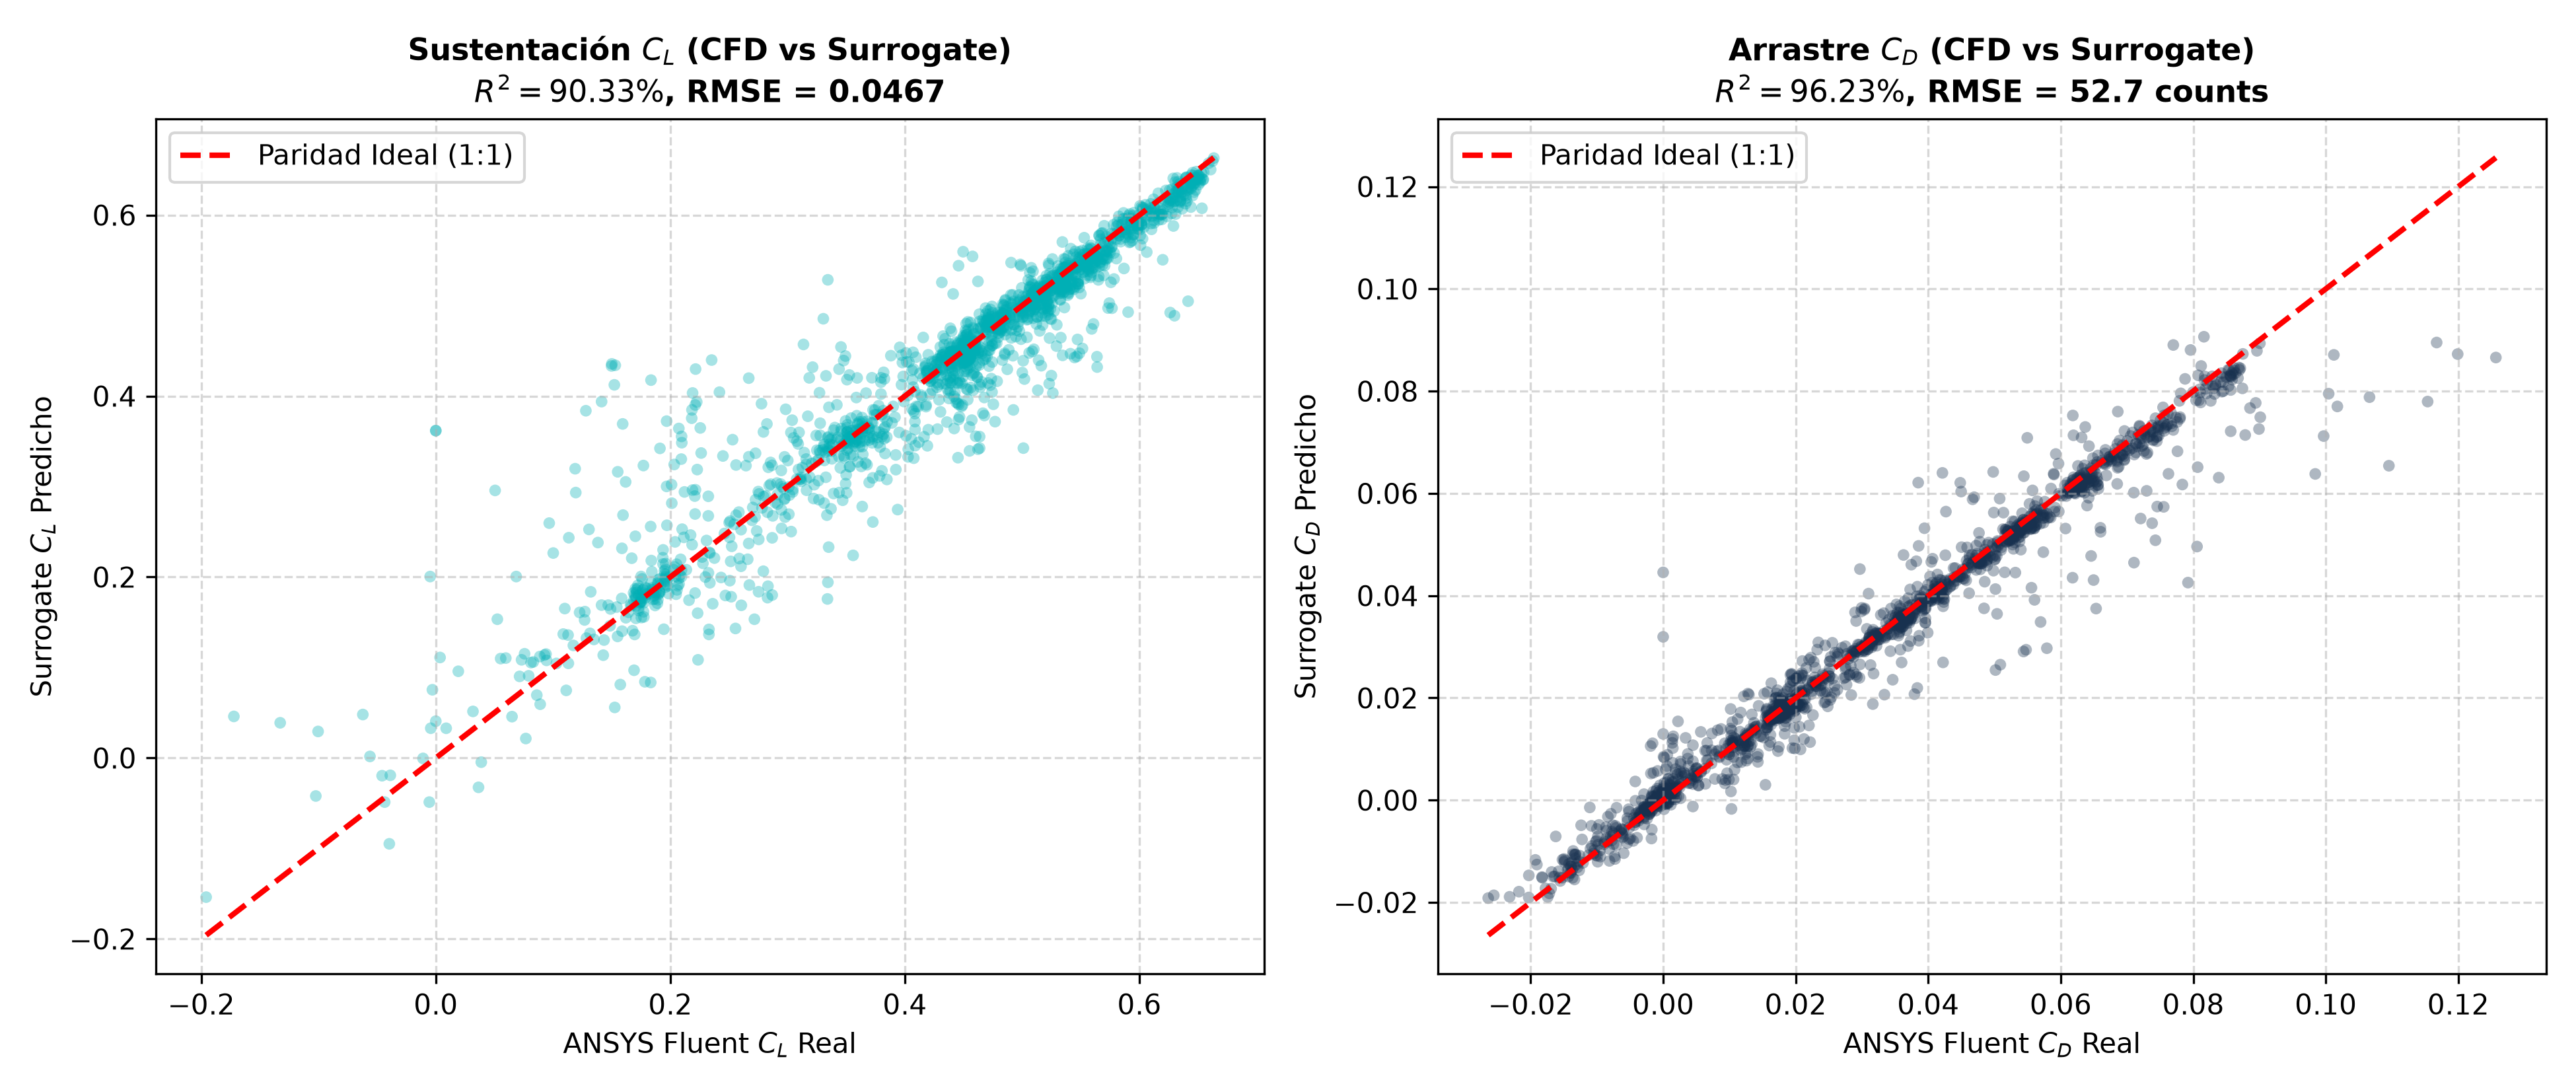
\includegraphics[width=0.95\textwidth]{../outputs/cfd_surrogate_parity_plots.png}
    \caption{Gráficos de paridad ($1:1$) del modelo sustituto de alta fidelidad frente a las simulaciones de ANSYS Fluent Transition-SST para $C_L$ (izquierda) y $C_D$ (derecha).}
    \label{fig:cfd_parity_plots}
\end{figure}

El ajuste del coeficiente de arrastre ($R^2 = 96.23\%$) demuestra que la red neuronal aprendió a modelar con alta fidelidad las pérdidas viscosas y de presión derivadas del engrosamiento de la burbuja laminar de transición a bajos números de Reynolds, superando la limitación histórica de subestimación de $C_D$ inherente a XFOIL.

\section{Configuración Experimental y Validación}
\label{sec:validacion}

El aporte diferencial de DIPAS radica en la cuantificación empírica de la brecha entre la simulación y la realidad. Una vez que el CVAE ha sido entrenado y genera perfiles óptimos para misiones específicas, se seleccionará la geometría más prometedora para su fabricación y ensayo.

\subsection{Parámetros de Diseño y Restricciones Físicas}
Basándose en las capacidades físicas del laboratorio y el túnel de viento, se adoptan los siguientes valores de referencia para el dimensionamiento del modelo de prueba y el acondicionamiento geométrico:
\begin{table}[htbp]
\centering
\caption{Supuestos técnicos y limitaciones operativas para el modelo de validación.}
\label{tab:supuestos_tunel}
\begin{tabular}{lll}
\toprule
\textbf{Parámetro} & \textbf{Valor Asumido} & \textbf{Origen / Justificación} \\
\midrule
Cuerda del modelo ($c$) & $200\text{ mm}$ & Ensayo 2D en sección de ensayo típica \\
Velocidad del aire ($V$) & $10\text{ a }30\text{ m/s}$ & Caracterización operativa del túnel \\
Rango de Reynolds ($Re$) & $\sim 130.000\text{ a }400.000$ & Aire a $20^\circ\text{C}$ con $c=200\text{ mm}$ \\
Instrumentación principal & Balanza de fuerzas y tomas de $C_p$ & Sensores piezoeléctricos discretos \\
Espesor mín. borde de fuga & $0,6\text{ mm}$ & Límite de fabricación por impresión FDM \\
\bottomrule
\end{tabular}
\end{table}

\subsection{Validación de Presión Discreta ($C_p$)}
Además de contrastar los coeficientes globales integrados ($C_L, C_D$), se propone extraer la distribución espacial discreta de los coeficientes de presión ($C_p$) obtenidos de la simulación CFD RANS (AirfRANS) en las coordenadas relativas de cuerda ($x/c$) donde se encuentran ubicados físicamente los sensores de presión piezoeléctricos del modelo. Esta validación puntual permite detectar localmente fenómenos como la posición de la burbuja de laminación y el punto de transición del flujo sin necesidad de entrenar al CVAE con campos de flujo completos.

\subsection{Preguntas Técnicas a Validar con la Cátedra}
Para cerrar los supuestos de la Tabla~\ref{tab:supuestos_tunel}, se plantea el siguiente cuestionario técnico para discutir con el cuerpo docente de Aerodinámica II:
\begin{enumerate}
    \item \textbf{Efectos de Bloqueo}: ¿Es adecuado el tamaño de cuerda de $200\text{ mm}$ para evitar el bloqueo del túnel en ensayos bidimensionales con paneles laterales?
    \item \textbf{Rango de Ensayos}: ¿Cuál es la velocidad óptima para obtener lecturas estables en la balanza mecánica/digital sin exceder las cargas estructurales de los soportes?
    \item \textbf{Tomas de Presión y Maquetado}: ¿Qué número de sensores piezoeléctricos se disponen y en qué coordenadas exactas de cuerda ($x/c$) están ubicadas las tomas? ¿Debemos diseñar la geometría con conductos internos en CAD para acoplar tomas metálicas durante la impresión 3D?
    \item \textbf{Eje de Soporte}: ¿Cuál es el sistema de anclaje físico del modelo al marco del túnel (por ejemplo, barra pasante o soportes laterales) y a qué distancia de la cuerda se localiza el eje de cabeceo?
\end{enumerate}


\newpage
\bibliographystyle{IEEEtran}
\bibliography{references}

\end{document}
